\chapter{Множества} 

%sets: prefix
Множество --- фундаментальное понятие всей дискретной математики. Для углубленного изучения рекомендуются \cite{bib:sudoplatov:discrmath, bib:haggard:discrmathprogrammer, bib:novic:discrmathprogrammer}.


\section{Базовые понятия теории множеств}

Множество --- фундаментальное понятие. Оно не определимо явно. Под множеством $M$ подразумевается совокупность некоторых объектов, которые будут называться \emph{элементами} множества $M$. Принадлежность элемента $x$ множеству $M$ обозначается символом $\in$. Пишут $x\in M$, если $x$ является элементом множества $M$, и $x\not\in M$, если $x$ не является элементом $M$. 

Чтобы задать множество, нужно указать какие элементы ему принадлежат. Для этого существует несколько способов.
\begin{itemize}
    \item Явным перечислением элементов:\[\{a_1,a_2,\ldots,a_n\}.\]
    \item Характеристическим предикатом:\[\{x|P(x)\}.\]
    \item Порождающей процедурой:\[\{x|x=f\}.\]
\end{itemize}

\begin{exampl} Способы задания множеств

    \begin{itemize}
        \item Явное перечисление:$M=\{a,b,c,d\}$. Элементами множества могут быть другие множества $M=\{1,\{2,3\},\{4,5\}\}$.
        \item Характеристический предикат, задающий множество четных чисел:$M=\{x|x\text{---четное}\}$.
        \item Порождающая процедура:$M=\{n|for\ n=1\ to\ 4\ do\ yeld\ n;\}$. Генерируется множество $M=\{1,2,3,4\}$.
    \end{itemize}
\end{exampl}

%Характеристический предикат является хорошим способом задать множество, но с его формулировкой нужно быть очень осторожным. Рассмотрим, например, парадокс Рассела. Рассмотрим множество всех множеств, не содержащих себя в качестве элемента.
%\[Y=\{X|X\not\in X\}\]
%Зададимся вопросом является ли $Y$ элементом самого себя? Если $Y$ не содержит себя в качестве элемента, то оно по определению должно являться элементом самого себя. Если $Y$ является элементом самого себя, то в этом случае по условию оно само себя в качестве элемента содержать не может.

Существуют некоторые множества, для которых приняты стандартные обозначения:
\begin{itemize}
    \item $\emptyset=\{\}$ --- пустое множество;
    \item $\mathbb{N}=\{0,1,2,\ldots\}$ --- множество натуральных чисел;
    \item $\mathbb{Z}=\{0,\pm 1,\pm 2,\ldots\}$ --- множество целых чисел;
    \item $\mathbb{Q}$ --- множество всех рациональных дробей;
    \item $\mathbb{P}$ --- множество простых чисел;
    \item $\mathbb{R}$ --- множество вещественных (действительных) чисел;
    \item $\mathbb{C}$ --- множество комплексных чисел.
\end{itemize}

Множество $A$ \emph{содержится} в множестве $B$ (множество $B$ \emph{включает} множество $A$), если каждый элемент $A$ есть элемент $B$. Такое отношение между множествами $A$ и $B$ называется \emph{отношением нестрогого включения} и обозначается символом $\subseteq$:
\[A\subseteq B, \text{если\ } (x\in A)\Rightarrow (x\in B).\]
В этом случае $A$ --- \emph{подмножество}, а $B$ --- \emph{надмножество}. Запись $B\supseteq A$ обозначает то же, что и запись $A\subseteq B$.

Множество $A$ называется \emph{собственным} подмножеством множества $B$, если $A$ является подмножеством множества $B$, и если $B$ не является подмножеством $A$. Такое отношение между множествами $A$ и $B$ обозначается символом \emph{отношения строгого включения} $\subset$:
\[A\subset B,\text{если $(A\subseteq B)\land(B\not\subseteq A)$},\]
где $\land$ --- обозначение
\footnote{
    В различных литературных источниках основные логические связки обозначаются по разному. Например.
    \begin{itemize}
        \item Объединение условий по <<И>>: <<$\&$>>, <<$\land$>>. Перечисление условий через запятую также считается объединением по <<И>>:$A,B,C$, например, соответствует $A\land B\land C$.
        \item Объединение условий по <<ИЛИ>>: <<$\lor$>>, <<$|$>>, <<$||$>>.
        \item Логическое отрицание условия $A$: $\lnot A$, $\bar{A}$.
    \end{itemize}
} объединения логических условий по <<И>>. Запись $B\supset A$ означает то же, что и запись $A\subset B$.
  
Для любого множества $M$ справедливо:
\begin{itemize}
    \item $M\subseteq M$;
    \item $\emptyset\subseteq M$.
\end{itemize}

Множества $A$ и $B$ равны (обозначается $A=B$), если $A$ подмножество $B$ и $B$ подмножество $A$:

\begin{equation}
    \label{eq:ABSetEquality}
    (A=B)\Leftrightarrow(A\subseteq B\land B\subseteq A).
\end{equation}

Множества $A$ и $B$ находятся в \emph{общем положении} (обозначается $\text{ОП}(A,B)$), если одновременно выполняются три условия (см. рис.\ref{fig:commonABset}):
\begin{enumerate}
    \item $\exists x (x\in A \land  x\not\in B)$,
    \item $\exists y (y\in B \land  y\not\in A)$,
    \item $\exists z (z\in A \land  z\in B)$.
\end{enumerate}

\begin{figure}
    \centering
    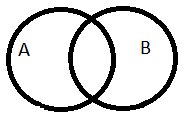
\includegraphics{fig/commonABset}
    \caption{Общее положение множеств $A$ и $B$}
    \label{fig:commonABset}
\end{figure} 

Два множества $A$ и $B$ могут находится лишь в одном из следующих отношений:
\begin{enumerate}
    \item $A=B$;
    \item $A\subset B$;
    \item $A\supset B$;
    \item $A\cup B = \emptyset$, т.е. $A$ и $B$ не имеют общих элементов;
    \item $\text{ОП}(A,B)$, т.е. $A$ и $B$ находятся в общем положении. 
\end{enumerate}

Количество элементов в \emph{конечном} множестве $A$ называют \emph{мощьностью конечного множества} и обозначают $|A|$.

Множество всех подмножеств множества $M$ называется \emph{булеаном} и обозначается $2^M$:
\[2^M=\{A|A\subseteq M\}.\]
Для конечного множества $M$ справедливо $\left|2^M\right|=2^{\left|M\right|}$.

В алгебре множеств вводятся следующие \emph{основные} операции над множествами (см. рис. \ref{fig:mainSetOperations}):
\begin{enumerate}
    \item объединение:\[A\cup B=\{x|x\in A \lor x\in B\};\]
    
    \item пересечение:\[A\cap B=\{x|x\in A \land x\in B\};\]
    
    \item дополнение:\[\overline{A}=\{x|x\not\in A\}.\]
\end{enumerate}

\begin{figure}
    \centering
    \begin{tabular}{||c||c||c||}
        \hline\hline
        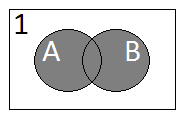
\includegraphics[width=.2\textwidth]{fig/ABsetOr}
            & 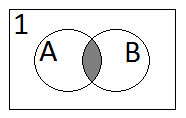
\includegraphics[width=.2\textwidth]{fig/ABsetAnd}
                & 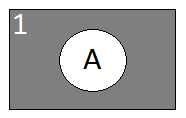
\includegraphics[width=.2\textwidth]{fig/AsetNot}\\
        $A\cup B$ 
            & $A\cap B$
                & $\overline{A}$\\
        \hline\hline
    \end{tabular}
    \caption{\emph{Основные} операции над множествами на диаграммах Венна}
    \label{fig:mainSetOperations}
\end{figure}

Кроме того, при выполнении преобразований над множествами удобно ввести следующие \emph{дополнительные} операции (см. рис. \ref{fig:slaveSetOperations}):
\begin{enumerate}
    \item разность:\[A\backslash B=A\cap\overline{B}=\{x|x\in A \land x\not\in B\};\]
    
    \item симметрическая разность:
    \[
    \begin{split}
        A\Delta B=(A\backslash B)\cup(B\backslash A)=(A\cup B)\backslash(A\cap B)=\\
        =\{x|(x\in A \land x\not\in B)\lor(x\not\in A\land x\in B)\}.
    \end{split}
    \]
\end{enumerate}

\begin{figure}
    \centering
    \begin{tabular}{||c||c||}
        \hline\hline
        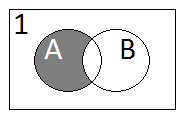
\includegraphics[width=.2\textwidth]{fig/ABsetSub}
            & 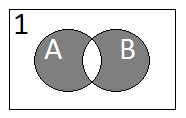
\includegraphics[width=.2\textwidth]{fig/ABsetSymSub}\\
        $A\backslash B$ 
            & $A\Delta B$\\
        \hline\hline
    \end{tabular}
    \caption{\emph{Дополнительные} операции над множествами на диаграммах Венна}
    \label{fig:slaveSetOperations}
\end{figure}

Операции над множествами обладают следующими свойствами:
\begin{enumerate}
    \item идемпотентность:
    \[A\cup A=A,A\cap A=A;\]
    
    \item коммутативность:
    \[A\cup B=B\cup A,A\cap B=B\cap A;\]
    
    \item ассоциативность:
    \[(A\cup B)\cup C=A\cup(B\cup C),(A\cap B)\cap C=A\cap(B\cap C);\]
    
    \item дистрибутивность:
    \[A\cup(B\cap C)=(A\cup B)\cap(A\cup C),A\cap(B\cup C)=(A\cap B)\cup(A\cap C);\]
    
    \item законы де Моргана:
    \[
        \overline{A\cap B}=\overline{A}\cup\overline{B},
        \overline{A\cup B}=\overline{A}\cap\overline{B};
    \]
    
    \item поглощение:
    \[(A\cup B)\cap A=A,(A\cap B)\cup A=A;\]
    
    \item свойства нуля (пустого множества $\emptyset$):
    \[(A\cup \emptyset)=A,(A\cap \emptyset)=\emptyset;\]
    
    \item свойства единицы (универсального множества $1$):
    \[(A\cup 1)=1,(A\cap 1)=A;\]
    
    \item инволютивность:
    \[\overline{\overline{A}}=A;\]
        
    \item свойства дополнения:
    \[
        \overline{A}\cup A=1,
        \overline{A}\cap A=\emptyset;
    \]
    
    \item выражение разности:
    \[
        A\backslash B=A\cap\overline{B}.
    \]
\end{enumerate}

Докажем некоторые утверждения
\begin{exampl} 
    Докажем закон инволютивности: $\overline{\overline{A}}=A$. 
\end{exampl}
\begin{proof}
    Исходя из определения равенства (формулы \eqref{eq:ABSetEquality}), докажем, что $\overline{\overline{A}}\subseteq A$ и $A\subseteq\overline{\overline{A}}$.
    \begin{enumerate}
        \item $\overline{\overline{A}}\subseteq A$. Допустим, $x\in\overline{\overline{A}}$, тогда $x\not\in\overline{A}$. Это значит, что $x\in A$.
        \item $A\subseteq\overline{\overline{A}}$. Допустим, $x\in A$, тогда $x\not\in\overline{A}$. Стало быть $x\in\overline{(\overline{A})}$.
    \end{enumerate}
\end{proof}

\begin{exampl} 
    Докажем (по формуле \eqref{eq:ABSetEquality}) закон де Моргана для случая $\overline{A\cup B}=\overline{A}\cap\overline{B}$. 
\end{exampl}
\begin{proof}
    Докажем, что $\overline{A\cup B}\subseteq\overline{A}\cap\overline{B}$ и $\overline{A}\cap\overline{B}\subseteq\overline{A\cup B}$.
    \begin{enumerate}
        \item $\overline{A\cup B}\subseteq\overline{A}\cap\overline{B}$. Возьмем элемент $x\in \overline{A\cup B}$. Делаем вывод, что $x\not\in A\cup B$. Поскольку элемент $x$ не входит в объединение множеств, то он не может входить ни в одно из этих множеств. Поэтому справедливо $x\not\in A$ и $x\not\in B$. То есть $x\in\overline{A}$ и $x\in\overline{B}$, по определению $x\in\overline{A}\cap\overline{B}$.
        \item $\overline{A}\cap\overline{B}\subseteq\overline{A\cup B}$. Возьмем элемент $x\in\overline{A}\cap\overline{B}$. Тогда $x\in\overline{A}$, а значит $x\not\in A$. Аналогично делаем вывод, что $x\not\in B$. Стало быть $x\not\in(A\cup B)$, а значит $x\in\overline{A\cup B}$.
    \end{enumerate}
\end{proof}

\begin{exampl}
    Докажем (по формуле \eqref{eq:ABSetEquality}), что операция разности множеств выражается через основные операции алгебры множеств так: $A\backslash B=A\cap\overline{B}$.
\end{exampl}
\begin{proof}
    Докажем, что $A\backslash B\subseteq A\cap\overline{B}$ и $A\cap\overline{B}\subseteq A\backslash B$.
    \begin{enumerate}
        \item $A\backslash B\subseteq A\cap\overline{B}$. Возьмем $x\in A\backslash B$, тогда по определению справедливо $x\in A$ и $x\not\in B$. То есть $x\in A$ и $x\in\overline{B}$. По определению $x\in A\cap\overline{B}$.
        \item $A\cap\overline{B}\subseteq A\backslash B$. Возьмем элемент $x\in A\cap\overline{B}$. Тогда справедливо $x\in A$ и $x\in\overline{B}$. То есть справедливо $x\in A$ и $x\not\in B$. По определению $x\in A\backslash B$.
    \end{enumerate}
\end{proof}

Следует отметить, что набор \emph{основных} операций алгебры множеств избыточен. Необходимым и достаточным минимумом операций являются, например, операции отрицания $\bar{~}$ и пересечения $\cap$. При этом операция объединения выражается через них: $A\cup B=\overline{\overline{A}\cap\overline{B}}$. Любую операцию алгебры множеств можно свести к указанным двум.

Впрочем, оказывается, что любую операцию алгебры множеств можно выразить лишь одной \emph{дополнительной} операцией вычитания:
\begin{itemize}
    \item $\overline{A}=1\backslash A$;
    \item $A\cap B=A\backslash (1\backslash B)$;
    \item $A\cup B=1\backslash((1\backslash A)\backslash B)$.    
\end{itemize}

Покажем, как на основе свойств операций над множествами можно проводить аналитические преобразования.
\begin{exampl}[Аналитические преобразования множеств]
\[
\begin{split}
A\backslash ((A\cup B)\backslash B) = A\cap\overline{((A\cup B)\cap\overline{B})}=\\
=A\cap(\overline{(A\cup B)}\cup\overline{\overline{B}})=A\cap((\overline{A}\cap\overline{B})\cup B)=\\
=A\cap((\overline{A}\cup B)\cap\underbrace{(\overline{B}\cup B)}_1)=A\cap (\overline{A}\cup B) = \underbrace{(A\cap\overline{A})}_\emptyset\cup(A\cap B)=\\
=A\cap B
\end{split}
\]
\qed
\end{exampl}

В завершение дадим несколько определений.

$\mathcal{E}=\{E_i|i\in\mathbb{N}\land E_i\subset M\}$ называется \emph{семейством} подмножеств множества $M$. Cемейство $\mathcal{E}$ называют \emph{покрытием} множества $M$, если каждый элемент $M$ содержится хотя бы в одном $E_i$:
\[
M\subseteq\bigcup_{i\in\mathbb{N}}E_i
\Leftrightarrow
\forall x\in M~\exists i\in\mathbb{N}~x\in E_i
\]

Семейство $\mathcal{R}$ называют \emph{дизъюнктивным} (или \emph{разбиением}), если множества $E_i$ попарно не пересекаются:
\[
\forall i,j\in\mathbb{N}~i\neq j\Rightarrow E_i\cap E_j=\emptyset
\]

Упорядоченную последовательность из $n$ элементов $(x_1,x_2,\ldots,x_n)$ будем называть \emph{кортежем} длины $n$. Элемент $x_i$ называется $i$-й \emph{координатой} кортежа. Два кортежа длины $n$: $(x_1,x_2,\ldots,x_n)$ и $(y_1,y_2,\ldots,y_n)$ равны тогда и только тогда, когда $x_1=y_1$,$x_2=y_2$,\ldots,$x_n=y_n$.

\emph{Декартовым} (прямым) произведенем множеств $A_1,A_2,\ldots,A_n$ называется множество 
\[\{(x_1,x_2,\ldots,x_n)|x_1\in A_1,x_2\in A_2,\ldots,x_n\in A_n\},\]
обозначаемое через 
\[A_1\times A_2\times\cdots\times A_n \text{~или~} \prod_{i=1}^{n}A_i.\]

Необходимо отметить, что $A\times B\neq B\times A$. 

Если $A_1=A_2=\ldots=A_n=A$, то множество $A_1\times A_2\times\cdots\times A_n$ называется $n$-й степенью множества $A$  и обозначается как $A^n$. По определению положим $A^0=\{\emptyset\}$.

\begin{exampl}
    Для множеств $A=\{a,b\}$ и $B=\{1,2\}$ имеем:
    \begin{itemize}
        \item $A\times B=\{(a,1),(b,1),(a,2),(b,2)\}$;
        \item $B\times A=\{(1,a),(1,b),(2,a),(2,b)\}$;
        \item $A\times A=A^2=\{(a,a),(a,b),(b,a),(b,b)\}$.
    \end{itemize}
    \qed
\end{exampl}

\begin{exampl}Щахматная доска.
    Пусть 
    \[
        A=\{a,b,c,d,e,f,g,h\},
        B=\{1,2,3,4,5,6,7,8\},
    \]
            тогда множество пар $(x,y)\in A\times B$ --- множество клеток шахматной доски.
    \qed
\end{exampl}

%TODO представление множеств в компьютере
%Множество из n>8 элементов. Представляется массивом байт. Написать алгоритм проверки наличия m-го элемента множества.
%Массив из скольки байт потребуется для представления $n$-элементного множества. Следует использовать операцию целочисленного деления 


\section*{Задания}
\addcontentsline{toc}{section}{Задания}

\begin{enumerate}
    \item Перечислить элементы указанных множеств. Определить мощность каждого множества.
    \begin{enumerate}
        \item $\emptyset$
        
        \item $\{\emptyset\}$
        
        \item $\{a,\{b,c\},d\}$
        
        \item $\{p|p\in \mathbb{P} \land 7\leq p\leq 30\}$
        
        \item $2^{\emptyset}$
        
        \item $2^{\{1,\{2,3\},\{4,5\}\}}$
        
        \item Числа Фибоначчи определяются рекурсивно так: 
        \[f(k)=
            \begin{cases}
            f(0)=1,\\
            f(1)=1,\\
            f(k)=f(k-1)+f(k-2),\text{при $k\in\mathbb{N}\land k>1$}.
            \end{cases}
        \]
        Определить $\{n|n=f(k),k\in\mathbb{N},4\leq n\leq 40\}$        
    \end{enumerate}
    
    \item Привести три возможных описания элементов множества $\{2,5,8,11,14\}$
    
    \item Задать множество точек, лежащих на сторонах треугольника с вершинами $A(0,0),B(0,3),C(4,0)$.
    
    \item Перечислить элементы следующих множеств.
    \begin{enumerate}
        \item $\{x|x\in\mathbb{Z}\land 6x^2+x-1=0\}$
        \item $\{x|x\in\mathbb{R}\land 6x^2+x-1=0\}$
        \item $\{x|x\in\mathbb{C}\land x^2+2x+2=0\}$
    \end{enumerate}
    
    \item Указать в каких отношениях находятся множества
    \begin{enumerate}
        \item $\{0,1\}$ и $\{2,3\}$
        \item $\{0,1\}$ и $\{0,1,2,3\}$
        \item $\{0,1,1\}$ и $\{1,0\}$
        \item $\{-1,0,1\}$ и $\mathbb{N}$
        \item $\mathbb{Z}$ и $\mathbb{R}$
        \item $\mathbb{C}$ и $\mathbb{R}$
        \item $\mathbb{Z}\backslash\{n|n=-k\land k\in\mathbb{N}\}$ и $\mathbb{N}$
    \end{enumerate}
    
    \item Даны множества $A=\{2,5,6,7\}$, $B=\{1,4,6,7\}$, $C=\{3,4,5,7\}$. Найти
    \begin{enumerate}
        \item $A\cap B$
        \item $A\cup B$
        \item $A\cap \overline{C}$
        \item $(A\cup B)\cap C$
        \item $A\backslash B$
        \item $A\Delta B = (A\cap \overline{B})\cup(B\cap\overline{A})$
    \end{enumerate}
    
    \item Рассмотрим три подмножества слов из словаря русского языка:
    \[A=\{x|x\text{---слово, стоящее перед словом <<собака>>}\}\]
    \[B=\{x|x\text{---слово, стоящее после слова  <<кошка>>}\}\]
    \[C=\{x|x\text{---слово, содержащее удвоенную букву}\}\]
    Какие из следующих выражений истинны?
    \begin{enumerate}
        \item $C\subset(A\cup B)$
        \item $\text{<<бассейн>>}\in (\overline{B}\cap C)$
        \item $\text{<<лассо>>}\in (B\Delta C)$
        \item $A\cap B=\emptyset$
    \end{enumerate}
    Опишите словесно свойства элементов следующих множеств:
    \begin{enumerate}
        \item $A\cap B \cap C$
        \item $(A\cup B)\cap \overline{C}$
    \end{enumerate}
    
    \item Пусть $A=\{n|n\in \mathbb{N} \land n=2k+1 \land k\in \mathbb{N}\}$,$B=\{n|n\in \mathbb{N} \land n=4k+1 \land k\in \mathbb{N}\}$. Доказать: 
    \begin{enumerate}
        \item $35\in A$
        \item $35\not\in B$
        \item $B\subseteq A$
        \item $B\subset A$
    \end{enumerate}
    
    \item Для множества $\{1,2,3,4\}$ постройте упорядоченный набор подмножеств, каждое последующее из которых отличается в одном элементе от предыдущего.
    
    \item Проиллюстрируйте диаграммами Венна для множеств $A,B,C$, находящихся в общем положении (см. рис. \ref{fig:commonABCset}).
    \begin{enumerate}
        \item $(A\backslash B)\cap C$
        \item $(A\backslash B)\cup C$
        \item $(A\backslash B)\cup (A\cap B)$
        \item $(A\cup B \cup C)\backslash(A\cap B\cap C)$
        \item $((A\cap B)\cup(A\cap C)\cup(B\cap C))\backslash(A\cap B\cap C)$
        \item $A\cap(\overline{B\cup C})$
    \end{enumerate}
    
    \item Записать эквивалентное выражение для выражения.
    \begin{enumerate}
        \item $A\cup B$, используя только операции $\cap,\bar{~}$.
        \item $A\backslash(B\cup C)$, используя только операции $\cap,\bar{~}$.
        \item $A\Delta B$, используя только операции $\cup,\bar{~}$.
        \item $\overline{A}$, используя только операцию $\backslash$.
        \item $A\cup B$, используя только операцию $\backslash$.
    \end{enumerate}
    
    \item Общее положение множеств $A,B,C$ изображено на диаграмме Венна (рис. \ref{fig:commonABCset}). Выразить формулами подмножества, изображенные на рис. \ref{fig:sets:ABCsubsets}
    
    \begin{figure}[h]
        \centering
        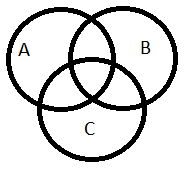
\includegraphics{fig/commonABCset}
        \caption{Общее положение множеств $A,B,C$}\label{fig:commonABCset}
    \end{figure} 
    
    \begin{figure}[!ht]
        \centering
        \begin{tabular}{||c||c||c||c||}
        \hline\hline
        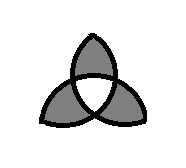
\includegraphics[width=.2\textwidth]{fig/ABCsubset1}
            & 
\includegraphics[width=.2\textwidth]{fig/ABCsubset2}
                & 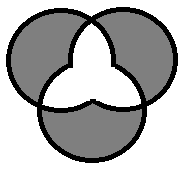
\includegraphics[width=.2\textwidth]{fig/ABCsubset3}
                    & 
\includegraphics[width=.2\textwidth]{fig/ABCsubset4}
                        \\
        а)  &б) &в) &г) \\ 
        \hline\hline
        \end{tabular}
        \caption{Подмножества общего положения $A,B,C$ на рис. \ref{fig:commonABCset}}
        \label{fig:sets:ABCsubsets}
    \end{figure} 
    
    \item Доказать, что на рисунке \ref{fig:sets:commonABCDset} изображено общее положение четырёх множеств. Обосновать, почему четырьмя кругами такое общее положение изобразить не получится?
    \begin{figure}[!ht]
        \centering
        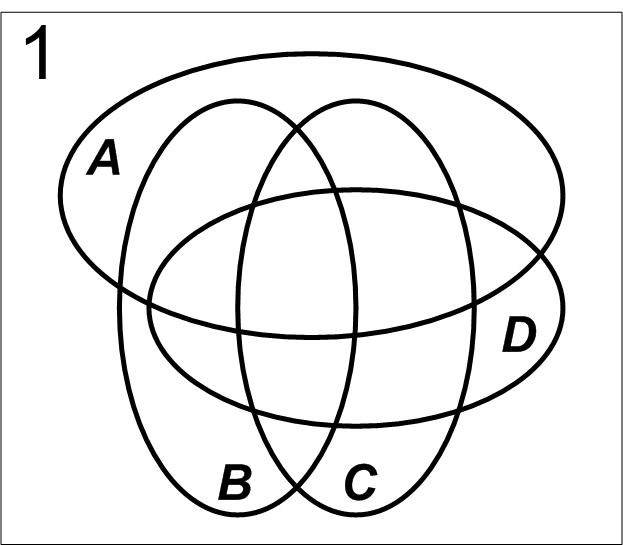
\includegraphics[width=.3\textwidth]{fig/commonABCDset}
        \caption{Общее положение четырёх множеств}
        \label{fig:sets:commonABCDset}
    \end{figure} 
    
    \item Доказать, что 
    \begin{enumerate}
        \item $(A\cap B)\cup A=A$
        \item Если $A\subseteq B$ или $A\subseteq C$, то $A\subseteq B\cup C$
        \item $(A\subseteq B)\Leftrightarrow (A\cap B=A)$
        \item $(A\subseteq B)\Leftrightarrow (\overline{B}\subseteq\overline{A})$
        \item $(A=B)\Leftrightarrow (\overline{A}=\overline{B})$
    \end{enumerate}
    
    \item Для $n$-элементного множества $A=\{a_1,\ldots,a_n\}$ оценить количество.
    \begin{enumerate}
        \item $n$-элементных кортежей, координаты которых принимают значения элементов $A$. Элементов множества $\{(x_1,\ldots,x_n)|x_1\in A,\ldots,x_n\in A\}$.
        
        \item $n$-элементных кортежей, координаты которых принимают значения элементов $A$, и при этом попарно различны. Элементов множества $\{(x_1,\ldots,x_n)|x_1\in A,\ldots,x_n\in A,\forall i,j i\neq j x_i\neq x_j, 1\leq i,j\leq n\}$.
        
        \item $m$-элементных кортежей ($m\leq n$), координаты которых принимают значения элементов $A$, и при этом попарно различны. Элементов множества $\{(x_1,\ldots,x_n)|x_1\in A,\ldots,x_n\in A,\forall i,j i\neq j x_i\neq x_j, 1\leq i,j\leq m\}$.
        
        \item $m$-элементных подмножеств множества $A$.
    \end{enumerate}
    
    \item Найти:
    \begin{enumerate}
        \item для множества $\{1,2,3,4\}$ все возможные двухэлементные подмножества;
        \item для множества $\{1,2,3,4\}$ все возможные трехэлементные подмножества;
        \item для множества $\{1,2,3\}$ все возможные трехэлементные кортежи, содержащие взаимно различные элементы $M$;
        \item для множества $\{1,2,3,4\}$ все возможные двухэлементные кортежи, содержащие взаимно различные элементы $M$;
    \end{enumerate}
    
    \item Определить количество $m$-элементных подмножеств $n$-элементного множества $\binom{m}{n}$. Сколько двухэлементных подмножеств 10 элементного множества? Чему равняется сумма $\sum_{i=0}^n \binom{i}{n}$?
    
    \item Является ли семейство $\mathcal{E}$ покрытием множества $M$? Дизьюнктивным покрытием (разбиением)?
    \begin{enumerate}
        \item $\mathcal{E}=\{\{a\},\{b,c\},\{c,d\}\}$, $M=\{a,b,c\}$.
        \item $\mathcal{E}=\{\{a\},\{b,c\},\{a,c\}\}$, $M=\{a,b,c\}$.
        \item $\mathcal{E}=\{\{a,b\},\{c\}\}$, $M=\{a,b,c\}$.
        \item $M=\mathbb{C}$,
        \[
        \begin{split}
            \mathcal{E}=\{
                \{a+b\cdot i|a,b\in\mathbb{R}\land b>0\land i=\sqrt{-1}\},\\
                \{a+b\cdot i|a,b\in\mathbb{R}\land b<0\land i=\sqrt{-1}\}
            \}.
        \end{split}
        \]
    \end{enumerate}
    
    \item Выполнить аналитические преобразования, применяя законы алгебры множеств.
    \begin{enumerate}
        \item $A\backslash((A\cup B)\backslash B)$
        \item $(A\backslash B)\cup(A\cap B)$
        \item $(A\cup B)\cap(A\cup\overline{B})\cap(\overline{A}\cup B)$
        \item $(A\cup (A\cap B))\cup(B\cap C)\cup(\overline{A}\cup C)$
        \item $A\cup\overline{(B\backslash\overline{A})}$
        \item $(A\cap B\cap C)\cup(\overline{A}\cap B\cap C)\cup\overline{B}\cup\overline{C}$
        \item $((A\cup B)\cap C)\cup(\overline{A}\cap C)\cup\overline{(\overline{B}\cup C)}$
        \item $(C\backslash(B\cap C))\cup((B\cap C)\cap(\overline{B}\cup\overline{C}))$
        \item $(\overline{A}\cup(A\cap B))\cup(\overline{B}\cup(A\cap B))$
        \item $A\cap\overline{((A\cup B)\cap\overline{B})}$
        \item $((A\cap B)\cup(A\cap\overline{C}))\cup((B\cup\overline{C})\cap\overline{A})$
    \end{enumerate}
\end{enumerate}
